
In questo capitolo presentiamo la metodologia seguita per il design e la creazione delle applicazioni CAMUS, utilizzando un approccio di visual programming dei mashup. Abbiamo scelto di mettere l'utente finale al centro della nostra progettazione, tenendo conto delle sue esigenze di utilizzo, cercando di mascherare la complessit� delle operazioni. %Esempio Viaggio???%
Nelle sezioni successive saranno esposti i problemi che abbiamo incontrato e le conseguenti scelte progettuali. 
\section{Architettura del sistema\label{sec:architettura-sistema}}




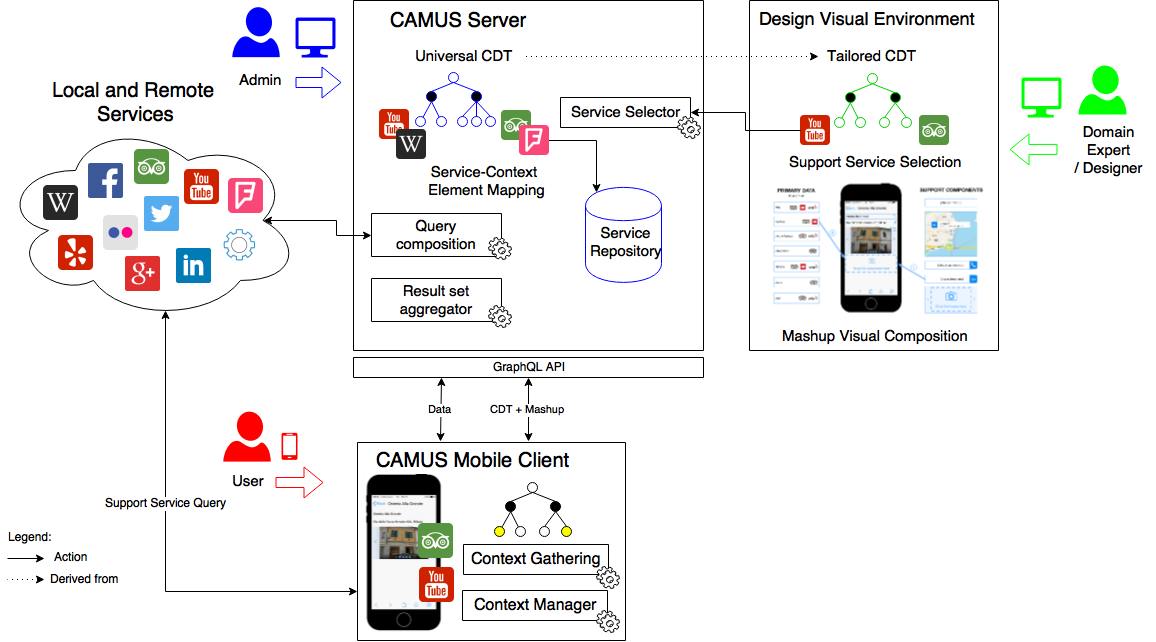
\includegraphics[width=\textwidth]{4-metodologia/Immagini/ArchitectureGen2016.png}

\section{Creazione dell'ecosistema dei servizi\label{sec:ecosistema-servizi}}

\textcolor{red}{Divisione tra servizi primari e di supporto}

\section{Universal CDT\label{sec:universal-cdt}}

\textcolor{red}{Spiegare come viene applicato il modello teorico in pratica\\
Divisione dei nodi filter e ranking\\
Divisione tra schema globale e tailored}

\section{Associazione dei servizi al CDT\label{sec:associazione-servizi-cdt}}

\textcolor{red}{Come vengono associati i servizi al contesto + ranking}

\section{Mashup Design\label{sec:mashup-design}}

\textcolor{red}{Spiegare lo schema per la generazione dinamica delle schermate\\
Descrizione web app per la creazione degli schemi}

\section{App Execution\label{sec:app-execution}}

\textcolor{red}{Interazione con l'app: flussi delle comunicazioni con il server (login, getPersonalData, contesto, ...)}